% Created 2017-07-03 Mon 00:00
% Intended LaTeX compiler: pdflatex
\documentclass[11pt]{article}
\usepackage[utf8]{inputenc}
\usepackage[T1]{fontenc}
\usepackage{graphicx}
\usepackage{grffile}
\usepackage{longtable}
\usepackage{wrapfig}
\usepackage{rotating}
\usepackage[normalem]{ulem}
\usepackage{amsmath}
\usepackage{textcomp}
\usepackage{amssymb}
\usepackage{capt-of}
\usepackage{hyperref}
\usepackage[margin=1in]{geometry}
\usepackage{multirow}
\renewcommand{\thesubsection}{\alph{subsection})}
\renewcommand{\thesubsubsection}{\alph{subsubsection})}
\author{Kevin Orr}
\date{July 2, 2017}
\title{Architecture Project 1}
\hypersetup{
 pdfauthor={Kevin Orr},
 pdftitle={Architecture Project 1},
 pdfkeywords={},
 pdfsubject={},
 pdfcreator={Emacs 25.2.2 (Org mode 9.0.8)}, 
 pdflang={English}}
\begin{document}

\maketitle

\section{ALPHA}
\label{sec:org1ee1864}
\subsection{Benchmark Results}
\label{sec:org14c85d8}
\begin{table}[htb]
\begin{center}
\begin{tabular}{|c|c|c|c|c|c|c|c|}
  \hline
  \multirow{3}{*}{Benchmark} & \multirow{3}{*}{Instructions} & \multicolumn{6}{c|}{Instruction Class Distribution} \\ \cline{3-8}
  & & \multirow{2}{*}{Load} & \multirow{2}{*}{Store} & Uncond & Cond   & Integer  & FP\\
  & &                       &                        & Branch & Branch & Math     & Math \\
  \hline
  \texttt{anagram.alpha} & 4940 & 18.24\% & 19.64\% & 6.30\% & 11.76\% & 43.59\% & 0.18\% \\
  \texttt{go.alpha} & 545823087 & 30.62\% & 8.17\% & 2.58\% & 10.96\% & 47.64\% & 0.03\% \\
  \texttt{compress95.alpha} & 88981 & 1.80\% & 78.53\% & 0.28\% & 5.76\% & 13.62\% & 0.00\% \\
  \texttt{cc1.alpha} & 337353488 & 24.67\% & 11.47\% & 4.12\% & 13.33\% & 46.30\% & 0.11\% \\
  \hline
\end{tabular}
\end{center}
\end{table}

\subsection{Is the benchmark memory- or computationally-intensive?}
\label{sec:org4260b6d}
\subsubsection{\texttt{anagram.alpha}}
\label{sec:orgeca32e3}
\textasciitilde{}38\% of the instructions are memory operations, and the rest are computational. This benchmark is mostly computationally-intensive.
\subsubsection{\texttt{go.alpha}}
\label{sec:orgd7fd98a}
This benchmark has the same approximate memory/computation ration as \texttt{anagram.alpha}, so it is mostly computationally-intensive.
\subsubsection{\texttt{compress95.alpha}}
\label{sec:org034678b}
This benchmark has \textasciitilde{}80\% memory operations; it is mostly memory-intensive.
\subsubsection{\texttt{cc1.alpha}}
\label{sec:org6ebda75}
This benchmark has only \textasciitilde{}36\% memory operations, with the rest computational. This is computationally-intensive.

\subsection{Is the benchmark mainly using integer or floating point computations?}
\label{sec:org0057d89}
\subsubsection{\texttt{anagram.alpha}}
\label{sec:org0b265ba}
43.59\% Integer vs 0.18\% FP, so FP.
\subsubsection{\texttt{go.alpha}}
\label{sec:orgd8d8009}
47.64\% Integer vs 0.03\% FP, so FP.
\subsubsection{\texttt{compress95.alpha}}
\label{sec:org0bebbf9}
13.62\% Integer vs 0.00\% FP, so FP.
\subsubsection{\texttt{cc1.alpha}}
\label{sec:org554dbf7}
46.30\% Integer vs 0.11\% FP, so FP.

\subsection{What \% of the instructions executed are conditional branches? How many instructions are computed between each pair of conditional branches?}
\label{sec:org4e1189a}
\subsubsection{\texttt{anagram.alpha}}
\label{sec:orgc38d898}
11.76\%. \(\Sigma\)(18.24\%, 19.64\%, 6.30\%, 43.59\%, 0.18\%)/11.76\% = 7.48
\subsubsection{\texttt{go.alpha}}
\label{sec:org3b97d90}
10.96\%. \(\Sigma\)(30.62\%, 8.17\%, 2.58\%, 47.64\%, 0.03\%)/10.96\% = 8.12
\subsubsection{\texttt{compress95.alpha}}
\label{sec:org112c281}
5.76\%. \(\Sigma\)(1.80\%, 78.53\%, 0.28\%, 13.62\%, 0.00\%)/5.76\% = 16.36
\subsubsection{\texttt{cc1.alpha}}
\label{sec:orgf94a670}
4.12\%. \(\Sigma\)(24.67\%, 11.47\%, 13.33\%, 46.30\%, 0.11\%)/4.12\% = 23.25

\section{Alpha vs PISA}
\label{sec:org2c048d6}
\subsection{ALPHA Benchmark Results}
\label{sec:orgabb86b8}
\begin{center}
\begin{tabular}{|c|c|c|c|c|c|c|c|}
  \hline
  \multirow{3}{*}{Benchmark} & \multirow{3}{*}{Instructions} & \multicolumn{6}{c|}{Instruction Class Distribution} \\ \cline{3-8}
  & & \multirow{2}{*}{Load} & \multirow{2}{*}{Store} & Uncond & Cond   & Integer  & FP\\
  & &                       &                        & Branch & Branch & Math     & Math \\
  \hline
  \texttt{test-math} & 49310 & 17.14\% & 10.44\% & 3.95\% & 11.03\% & 55.40\% & 1.88\% \\
  \texttt{test-fmath} & 19399 & 17.64\% & 12.58\% & 4.72\% & 11.17\% & 53.29\% & 0.43\% \\
  \texttt{test-llong} & 10527 & 17.66\% & 14.73\% & 5.47\% & 12.21\% & 49.63\% & 0.10\% \\
  \texttt{test-printf} & 983373 & 17.99\% & 10.74\% & 4.82\% & 11.39\% & 54.85\% & 0.09\% \\
  \hline
\end{tabular}
\end{center}

\subsection{PISA Benchmark Results}
\label{sec:orga30ce2a}
\begin{center}
\begin{tabular}{|c|c|c|c|c|c|c|c|}
  \hline
  \multirow{3}{*}{Benchmark} & \multirow{3}{*}{Instructions} & \multicolumn{6}{c|}{Instruction Class Distribution} \\ \cline{3-8}
  & & \multirow{2}{*}{Load} & \multirow{2}{*}{Store} & Uncond & Cond   & Integer  & FP\\
  & &                       &                        & Branch & Branch & Math     & Math \\
  \hline
  \texttt{test-math} & 213553 & 15.96\% & 10.67\% & 4.22\% & 13.84\% & 54.42\% & 0.88\% \\
  \texttt{test-fmath} & 53312 & 16.17\% & 14.47\% & 4.24\% & 15.08\% & 49.90\% & 0.11\% \\
  \texttt{test-llong} & 29495 & 16.38\% & 18.11\% & 4.37\% & 15.40\% & 45.70\% & 0.00\% \\
  \texttt{test-printf} & 1813745 & 19.22\% & 9.28\% & 5.13\% & 17.01\% & 49.33\% & 0.01\% \\
  \hline
\end{tabular}
\end{center}

\subsection{Comparison}
\label{sec:org474c407}
The PISA ISA requires many more (1.8x - 4.3x) instructions than the \mbox{ALPHA} ISA for the same programs.

\begin{center}
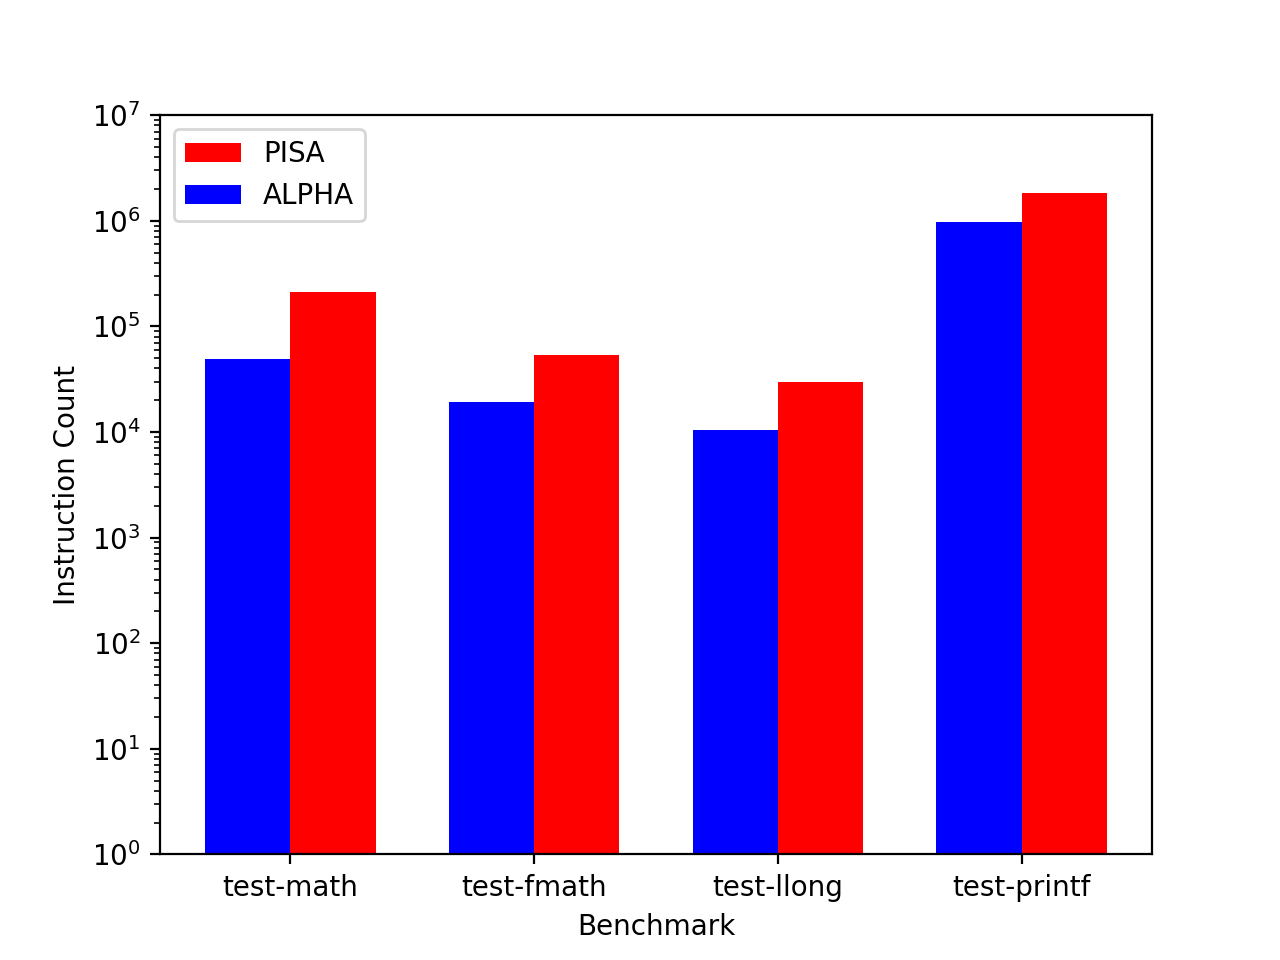
\includegraphics[width=.9\linewidth]{./bar_comparison.png}
\end{center}
\end{document}
